\documentclass[10pt,a4paper]{jsarticle}
\usepackage{listings,jlisting}
\usepackage{fancyhdr}
\usepackage{lastpage}
\usepackage[dvipdfmx]{graphicx,color}

\lhead{プログラミング実習IIレポート(第8回)}
\rhead{学籍番号:201811433 氏名:西田 直人}
\cfoot{\thepage/\pageref{LastPage}}

\pagestyle{fancy}

\title{プログラミングII実習レポート課題第8回}
\author{西田直人}

\begin{document}
%\markright{プログラミング実習1Aレポート(第1回) 学籍番号:201811433 氏名:西田直人}
%\maketitle
\begin{center}
{\LARGE プログラミング実習IIレポート課題第8回} \\
\large
西田直人 \\ 2019年1月28日
\end{center}
\normalsize
\section{課題8-1}

\subsection{source}
\lstinputlisting[basicstyle=\ttfamily\footnotesize,frame=single,breaklines=tr\
  ue,caption=a8-1.c]{a8-1.c}
\lstinputlisting[basicstyle=\ttfamily\footnotesize,frame=single,breaklines=tr\
  ue,caption=8-1Functions.c]{8-1Functions.c}
\lstinputlisting[basicstyle=\ttfamily\footnotesize,frame=single,breaklines=tr\
  ue,caption=Makefile1]{Makefile1}
\lstinputlisting[basicstyle=\ttfamily\footnotesize,frame=single,breaklines=tr\
  ue,caption=header1.h]{header1.h}


\subsection{result}

\begin{lstlisting}[basicstyle=\ttfamily\footnotesize,frame=single,breaklines=tr\
    ue]
  s1811433@LC2RR-P009:~/prog2/08/08kadai$ make -f Makefile1
  cc -c 8-1Functions.c header1.h
  cc -o a8-1 a8-1.o 8-1Functions.o
  s1811433@LC2RR-P009:~/prog2/08/08kadai$ make -f Makefile1 run
  ./a8-1

  >add 100 Sato
  add: no: 100, name: Sato

  >add 200 Yamamoto
  add: no: 200, name: Yamamoto

  >add 300 Imai
  add: no: 300, name: Imai

  >find Yamamoto
  no: 200, name: Yamamoto

  >find Kanamori
  ``Kanamori'' not found

  >del
  del: tail deleted

  >display
  no: 100, name: Sato
  no: 200, name: Yamamoto

  >save hoge.txt
  list saved in ``hoge.txt''

  >clear
  clear: list cleared

  >display
  (NULL)

  >load hoge.txt
  list loaded out of ``hoge.txt''

  >display
  no: 100, name: Sato
  no: 200, name: Yamamoto

  >add 400 Kato
  add: no: 400, name: Kato

  >display
  no: 100, name: Sato
  no: 200, name: Yamamoto
  no: 400, name: Kato

  >bye
  bye!
  s1811433@LC2RR-P009:~/prog2/08/08kadai$ 
     
\end{lstlisting}


\section{課題8-2}

\subsection{source}


\begin{lstlisting}[basicstyle=\ttfamily\footnotesize,frame=single,breaklines=tr\
    \
    ue]
  //構造体Point,ColoredCurveの定義

  typedef struct _point {
    int xi, yi;
    struct _point *next;
  } Point;


  typedef struct {
    Point *head;
    Point *tail;
    unsigned char r, g, b;
  } ColoredCurve;

\end{lstlisting}

\lstinputlisting[basicstyle=\ttfamily\footnotesize,frame=single,breaklines=tr\
  ue,caption=ColoredCurve.c]{ColoredCurve.c}

\lstinputlisting[basicstyle=\ttfamily\footnotesize,frame=single,breaklines=tr\
    ue,caption=Makefile2]{Makefile2}


\subsection{result}

\begin{figure}[h!]
  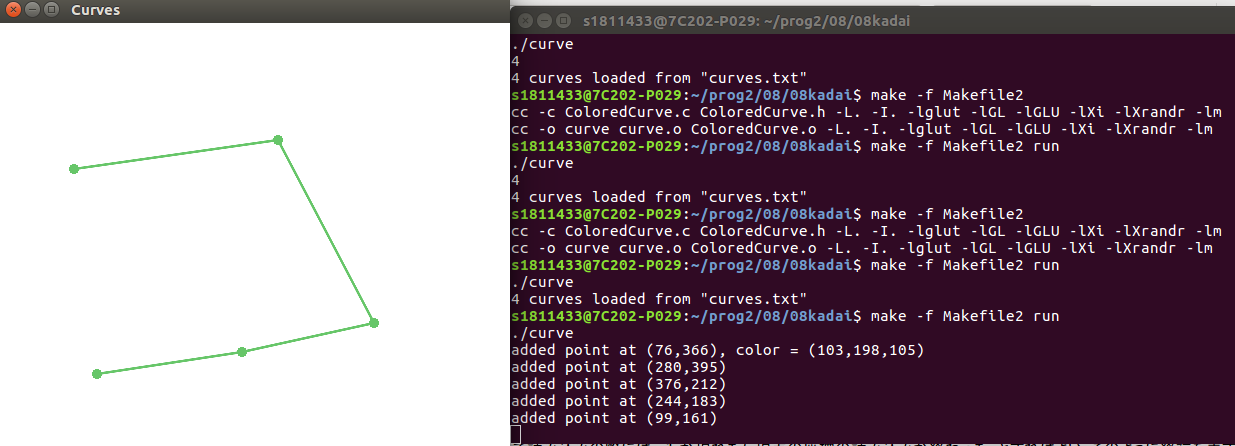
\includegraphics[width=0.8\linewidth]{01.png}
  \caption{クリックして折れ線の頂点を追加}
  \label{fig:sutehage}
\end{figure}

\begin{figure}[h!]
  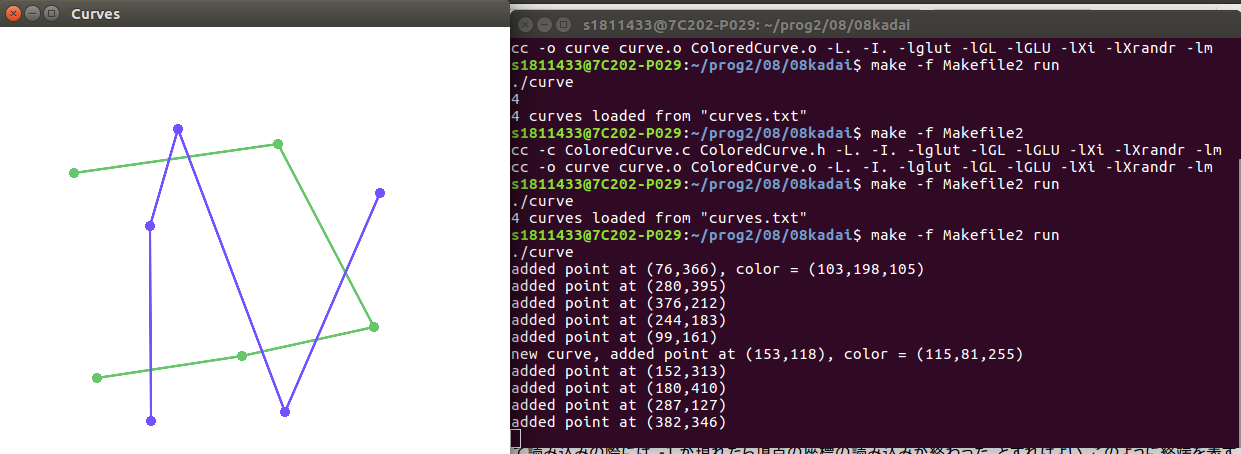
\includegraphics[width=0.8\linewidth]{02.png}
  \caption{Ctrl キー + クリックで新しい折れ線を開始}
  \label{fig:sutehage}
\end{figure}

\begin{figure}[h!p]
  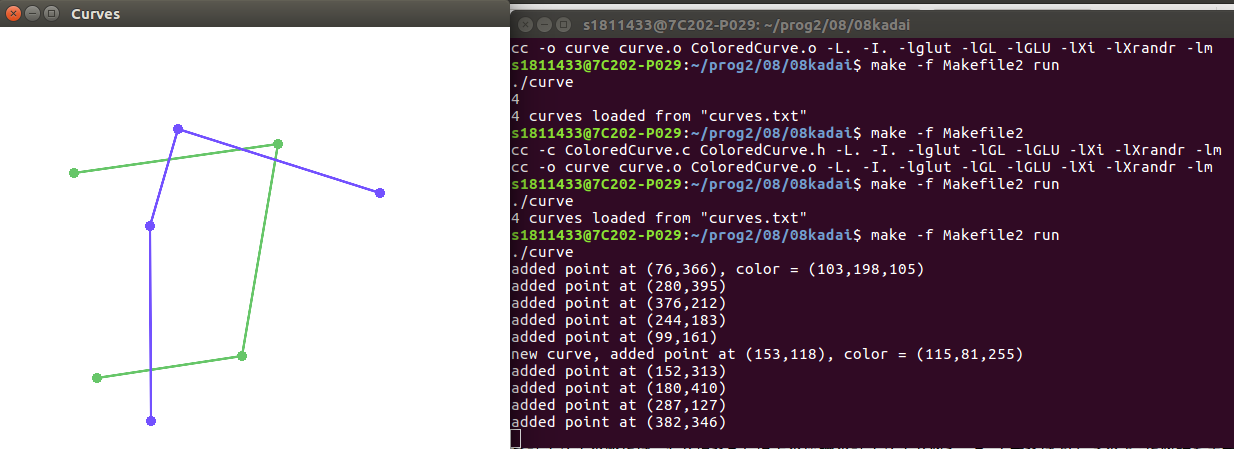
\includegraphics[width=0.8\linewidth]{03.png}
  \caption{Shift キー + クリックで頂点を削除}
  \label{fig:sutehage}
\end{figure}
\begin{figure}[h!p]
  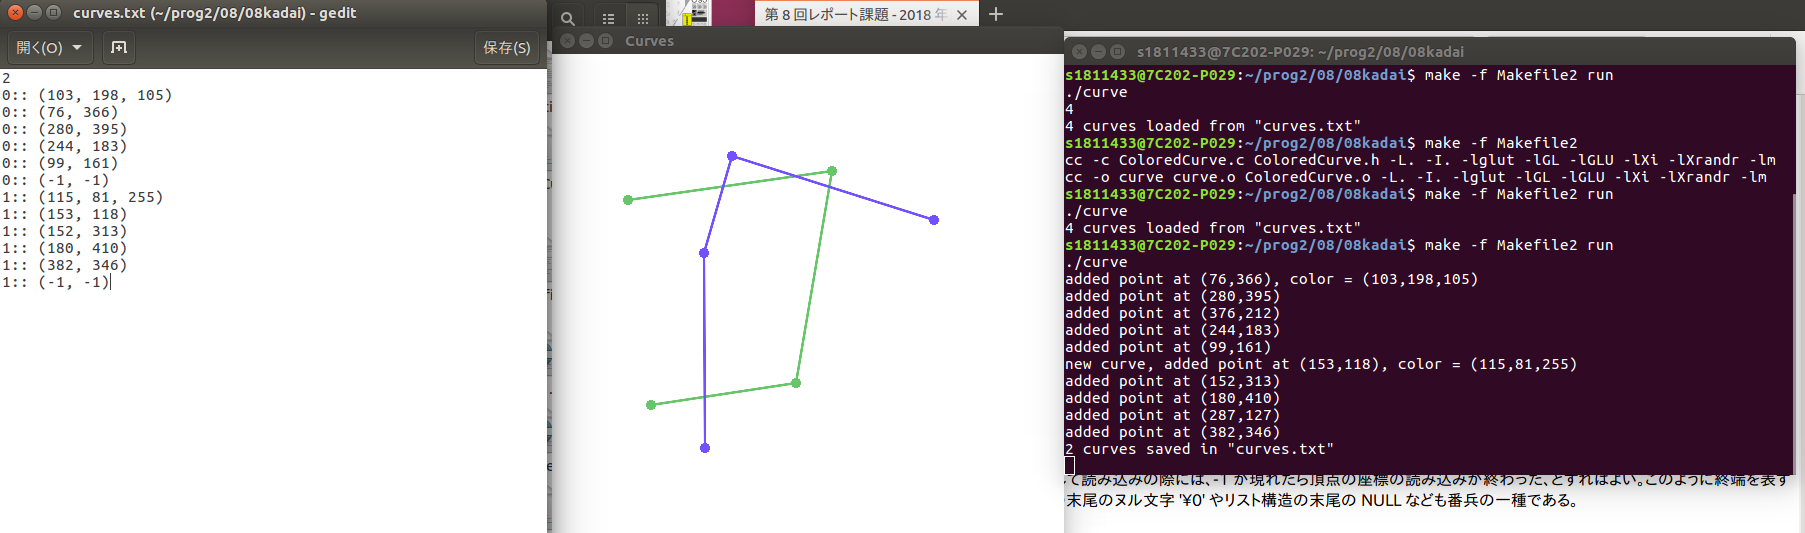
\includegraphics[width=0.8\linewidth]{04.png}
  \caption{sキーでファイルにデータを保存}
  \label{fig:sutehage}
\end{figure}
\begin{figure}[h!p]
  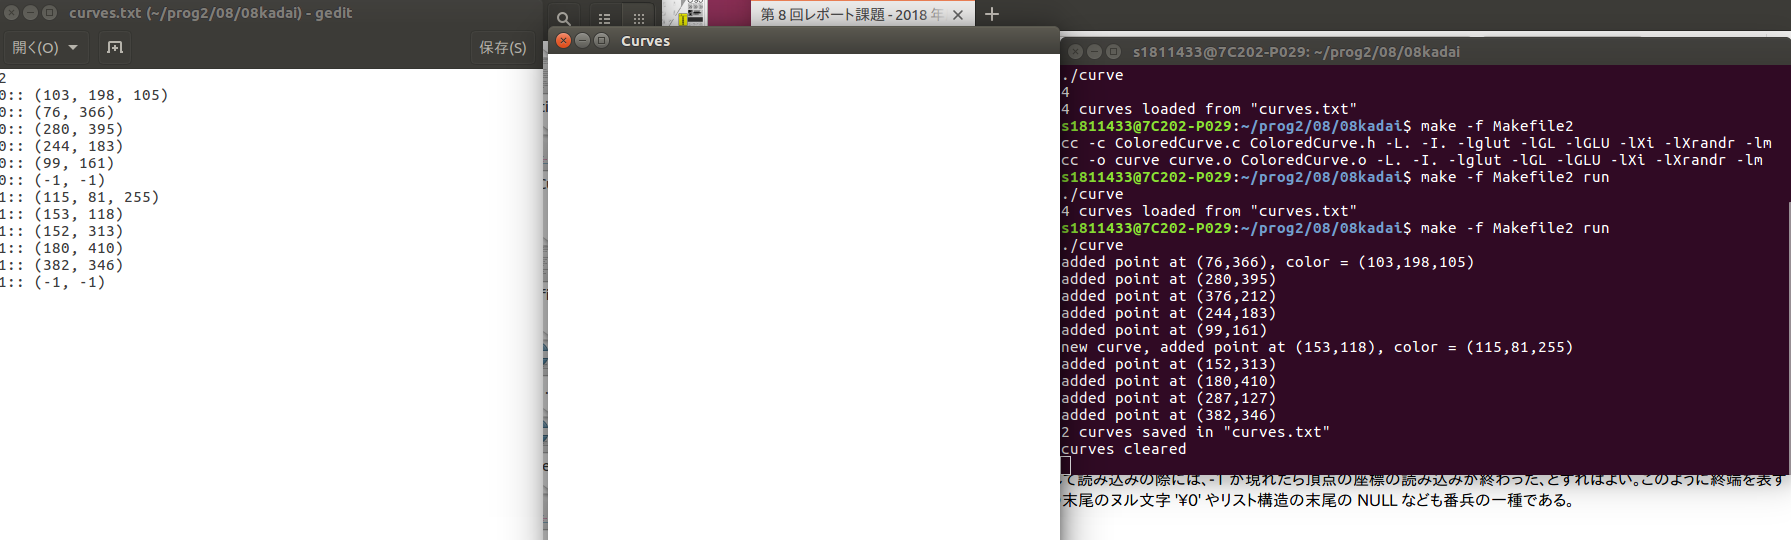
\includegraphics[width=0.8\linewidth]{05.png}
  \caption{スペースキーで描画を消去}
  \label{fig:sutehage}
\end{figure}
\begin{figure}[h!p]
  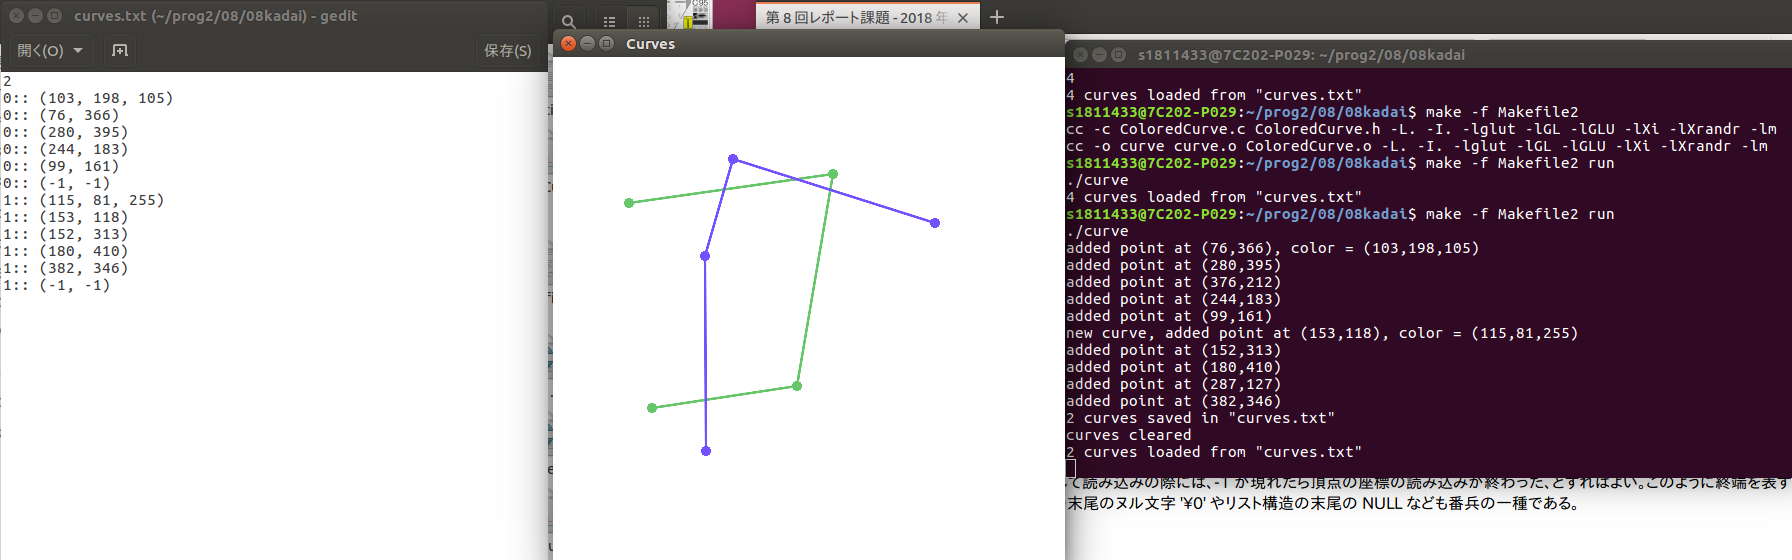
\includegraphics[width=0.8\linewidth]{06.png}
  \caption{lキーでファイルからデータを呼び出して描画}
  \label{fig:sutehage}
\end{figure}
\
\newpage
.
\newpage


\section{課題8-3}
\subsection{source}
this is a program for showing the result of some test data of everyone. I used 2-way structure.
\lstinputlisting[basicstyle=\ttfamily\footnotesize,frame=single,breaklines=tr\
ue,caption=a8-3.c]{a8-3.c}

\subsection{result}

\begin{lstlisting}[basicstyle=\ttfamily\footnotesize,frame=single,breaklines=tr\
  ue]
  s1811433@ubuntu:~/prog2/08/08kadai$ cc -o a8-3 a8-3.c
  s1811433@ubuntu:~/prog2/08/08kadai$ ./a8-3
  Experiment name: mast18の中でのテストスコアの比較
  participant no. 1
  name: Atarashi
  score:10
  N: nextdata
  P:previousdata
  Q:quit this program

  n
  participant no. 2
  name: Eisaki
  score:30
  N: nextdata
  P:previousdata
  Q:quit this program

  n
  participant no. 3
  name: Koroyasu
  score:40
  N: nextdata
  P:previousdata
  Q:quit this program

  n
  participant no. 4
  name: Tsukuda
  score:20
  N: nextdata
  P:previousdata
  Q:quit this program

  n
  participant no. 5
  name: Magome
  score:50
  N: nextdata
  P:previousdata
  Q:quit this program

  n
  participant no. 5
  name: Magome
  score:50
  N: nextdata
  P:previousdata
  Q:quit this program

  p
  participant no. 4
  name: Tsukuda
  score:20
  N: nextdata
  P:previousdata
  Q:quit this program

  p
  participant no. 3
  name: Koroyasu
  score:40
  N: nextdata
  P:previousdata
  Q:quit this program

  p
  participant no. 2
  name: Eisaki
  score:30
  N: nextdata
  P:previousdata
  Q:quit this program

  p
  participant no. 1
  name: Atarashi
  score:10
  N: nextdata
  P:previousdata
  Q:quit this program

  p
  participant no. 1
  name: Atarashi
  score:10
  N: nextdata
  P:previousdata
  Q:quit this program

  n
  participant no. 2
  name: Eisaki
  score:30
  N: nextdata
  P:previousdata
  Q:quit this program

  p
  participant no. 1
  name: Atarashi
  score:10
  N: nextdata
  P:previousdata
  Q:quit this program

  q
  s1811433@ubuntu:~/prog2/08/08kadai$ 
\end{lstlisting}

%\begin{figure}[h]
 % 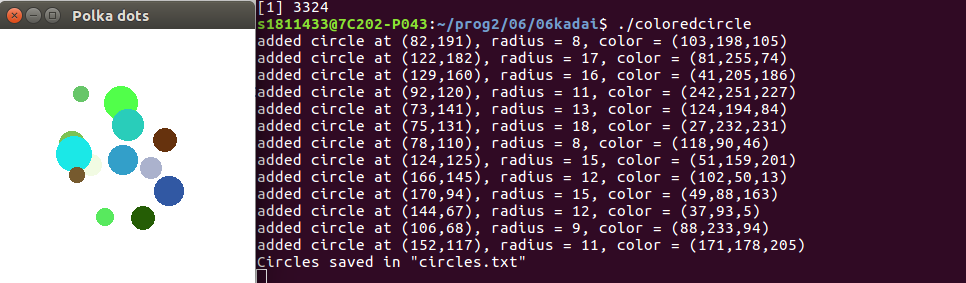
\includegraphics[width=0.8\linewidth]{b.png}
  %\caption{数回クリックしたあとにsを押した}
  %\label{fig:sutehage}
  
%\end{comment}
\end{document}
